\chapter{Resultados} 

Este capítulo se destina à apresentação dos resultados obtidos diante da implementação do algoritmo. Na primeira seção, há uma breve descrição da plataforma utilizada para adquirir as imagens. Na segunda seção são demonstrados os resultados obtidos no mapeamento das distorções com a variação de alguns parâmetros fixos. Já na terceira seção, é possível analisar os resultados de imagens já retificadas e, por fim, a quarta seção demonstra o resultado do mosaico obtido após os processamentos realizados na imagem.

\section{Plataforma de aquisição}

As aquisições das imagens foram realizadas em uma plataforma dedicada a fim de obter a maior controle das condições de aquisição. A câmera utilizada teve seus parâmetros automáticos desativados e a exposição foi configurada manualmente, a fim de evitar variações de iluminação entre as diferentes imagens. A câmera fixada um tripé e teve sua inclinação 
ajustada com auxilio de uma ferramenta de nível. Na Figura~\ref{fig:plataforma} é possível visualizar o ambiente onde foram realizados os ensaios.

\begin{figure}[htb]
    \caption{Plataforma utilizada para a aquisição das imagens. }
    \centering
    \vspace{.3cm}
    \begin{minipage}{.4\textwidth}
            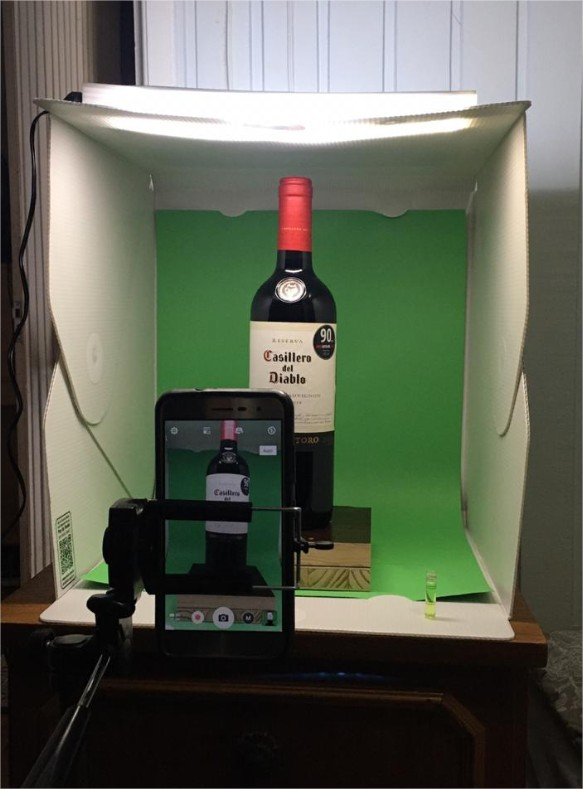
\includegraphics[width=\textwidth]{TCC/Imagens/plataforma.jpg}
            \fonte{O autor (2020).}
	\end{minipage}
    \label{fig:plataforma}
\end{figure}

\section{Identificação das distorções projetivas}

Com a identificação supervisionada dos seis pontos que representam os limites do rótulo efetuada, é necessário fazer o mapeamento das distorções a partir dessas delimitações. As distorções foram identificadas a partir do Algoritmo 1 (Mapeamento da Elipse) com uma escolha de trinta pontos horizontais, facilitando a visualização da caracterização geométrica do método. Na primeira execução, os parâmetros fixos do sistema foram dados por $R = 3,\!5$  e $d= 33$  (ambos em cm). Na Figura~\ref{fig:pontos_horizontal} é possível observar os resultados diante desta reprodução, onde os pontos em vermelho descrevem o mapeamento das distorções e os pontos em amarelo, as coordenadas que delimitam o rótulo.

\begin{figure}[htb]
    \caption{Aplicação do algoritmo para obtenção da distorção. }
    \centering
    \vspace{.3cm}
    \begin{minipage}{.3\textwidth}
      \centering
         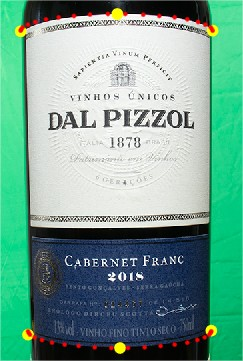
\includegraphics[width=\textwidth]{TCC/Imagens/pontos_horizontal.jpg}
            \fonte{O autor (2020).}
	\end{minipage}
    \label{fig:pontos_horizontal}
\end{figure}
    
O que se pode observar é que os pontos ficaram mais próximos entre si à medida que foram se aproximando do limite do rótulo (representando a distorção horizontal) e também atingiram um padrão geométrico esperado (elipse). As coordenadas restantes foram obtidas através do método descrito no capitulo anterior. Utilizando como parâmetro a presença de trinta pontos horizontais e vinte pontos verticais, a Figura~\ref{fig:total_distor} representa as distorções características a este rótulo perante o plano da imagem.

\begin{figure}[htb]
    \caption{Pontos que representam as distorções características desta garrafa.}
    \centering
    \vspace{.3cm}
    \begin{minipage}{.3\textwidth}
      \centering
         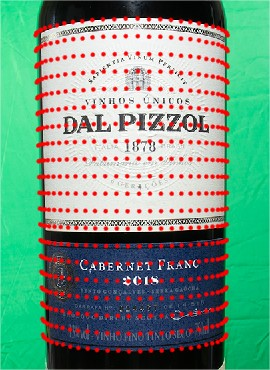
\includegraphics[width=\textwidth]{TCC/Imagens/total_distor.jpg}
            \fonte{O autor (2020).}
	\end{minipage}
    \label{fig:total_distor}
\end{figure}

Nota-se que as distorções mapeadas apresentaram uma característica muito fiel ao diagrama esquemático da Figura~\ref{fig:dist_vert}, onde as elipses de maior ordenada apresentam uma inclinação superior às elipses que se concentram mais próximas do centro do rótulo. Também é possível destacar que o sistema de mapeamento proposto em \cite{Lin:2013} considera que o eixo focal da câmera se encontra minuciosamente alinhado com o centro do rótulo. A alteração de parâmetros fixos ($R$ e $d$) influencia diretamente nos quesitos excentricidade das elipses extremas e, em consequência disso, das elipses internas.

\section{Remoção das distorções}

Para a validação desta etapa, a proposta de ensaio foi a utilização de uma garrafa envolvida por uma folha da papel quadriculado a fim de avaliar visualmente a retificação da imagem. Os desfechos a seguir demonstram o resultado da imagem planificada com diferentes quantidades de pontos verticais e pontos horizontais atribuídos. Na Figura~\ref{fig:ensaio_1a} é possível observar uma fotografia do objeto utilizado para a avaliação de resultados. Todas as execuções foram realizadas com valores ($N$) de pontos horizontais e verticais idênticos, proporcionando uma proporção de pontos de $N \times N$. 

\begin{figure}[ht]
    \caption{Imagem do objeto analisado.}
    \centering
    \vspace{.3cm}
    \begin{minipage}{.2\textwidth}
        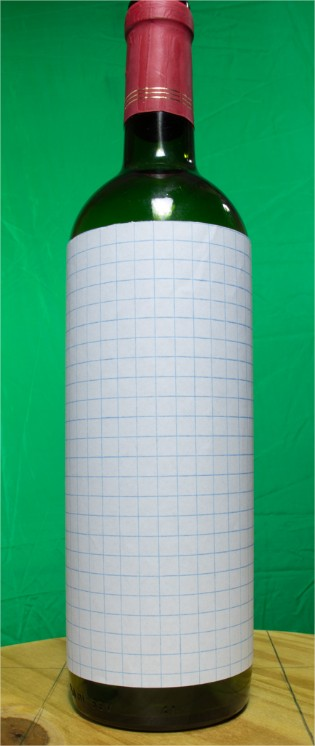
\includegraphics[width=\textwidth]{TCC/Imagens/ensaios/quadriculado.jpg}
        \fonte{O autor (2020).}
	\end{minipage}
    \label{fig:ensaio_1a}
\end{figure}

% \cred{<\textit{aqui ficou estranho... podes colocar resultados em anexo, mas não podes discutir os resultado aqui e colocar as imagens lá... acho melhor trazeres tudo para cá...}>}
A Figura~\ref{fig:ensaio_2_55a} demonstra o primeiro experimento, no qual
foi utilizado um valor de $N = 5$. A imagem à esquerda (a) representa a identificação das $N$ distorções encontradas em cada eixo, enquanto a imagem à direita (b) representa o resultado da imagem planificada. Entre a Figura~\ref{fig:ensaio_2_1010a} e a Figura~\ref{fig:ensaio_2_3030a}, os valores $N$ são dados por 10, 20 e 30, respectivamente, e apresentam a mesma estrutura de apresentação. O que se pode perceber nestes resultados é a melhoria significativa da representação planificada da imagem conforme o valor de $N$ é incrementado. No primeiro resultado, as falhas e distorções são facilmente visíveis conforme se aproximam do limite lateral da imagem. Contudo, os tamanhos dos retângulos são uniformes dentre a área mais central da imagem planificada. 

\begin{figure}[ht]
    \caption{Resultado da planificação com N = 5.}     
    \centering
    \vspace{0.3cm}
    \begin{minipage}{.5\textwidth}
      \centering
            \begin{tabular}{cc}
            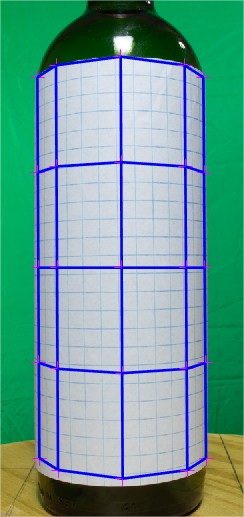
\includegraphics[width=.4\linewidth]{TCC/Imagens/ensaios/a_55.jpg} 
            &
            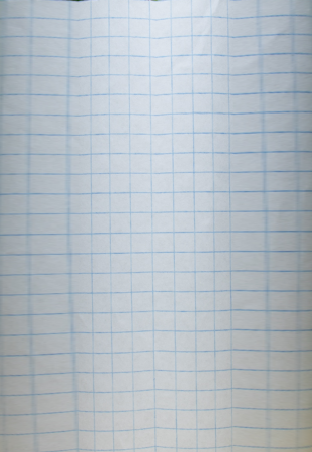
\includegraphics[width=.55\linewidth]{TCC/Imagens/ensaios/b_55.png}
            \\
            (a) Imagem original & (b) Imagem planificada.
            \end{tabular}
        \fonte{O autor (2020).}
	\end{minipage}
    \label{fig:ensaio_2_55a}
\end{figure}

\begin{figure}[ht]
    \caption{Resultado da planificação com N = 10.}     
    \centering
    \vspace{0.3cm}
    \begin{minipage}{.5\textwidth}
      \centering
            \begin{tabular}{cc}
            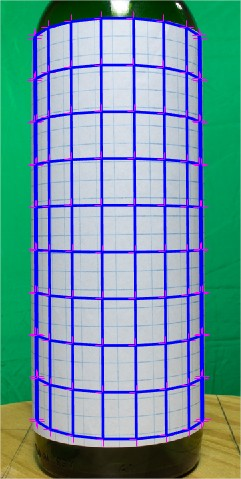
\includegraphics[width=.4\linewidth]{TCC/Imagens/ensaios/a_1010.jpg} 
            &
            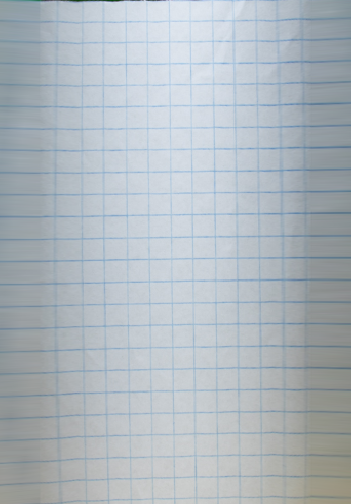
\includegraphics[width=.55\linewidth]{TCC/Imagens/ensaios/b_1010.png}
            \\
            (a) Imagem original & (b) Imagem planificada.
            \end{tabular}
        \fonte{O autor (2020).}
	\end{minipage}
    \label{fig:ensaio_2_1010a}
\end{figure}

No segundo experimento, apesar de uma melhor atribuição ao tamanho dos retângulos, ainda é possível destacar a presença de borrões. Além disso, o último retângulo de cada lado não apresenta uma última linha vertical, formando um retângulo maior. Por fim, os últimos dois experimentos se demonstraram sem a presença de deformações aparentes dentre as imagens resultantes. Todavia, é importante observar que com $N = 30$, apesar de pouco perceptível, a imagem apresenta a última linha vertical levemente mais visível e uniforme, se comparada ao caso em que $N = 20$.

\begin{figure}[ht]
    \caption{Resultado da planificação com N = 20.}     
    \centering
    \vspace{0.3cm}
    \begin{minipage}{.5\textwidth}
      \centering
            \begin{tabular}{cc}
            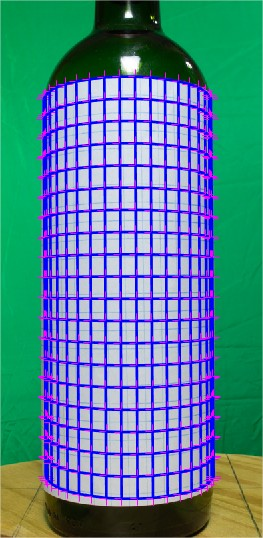
\includegraphics[width=.4\linewidth]{TCC/Imagens/ensaios/a_2020.jpg} 
            &
            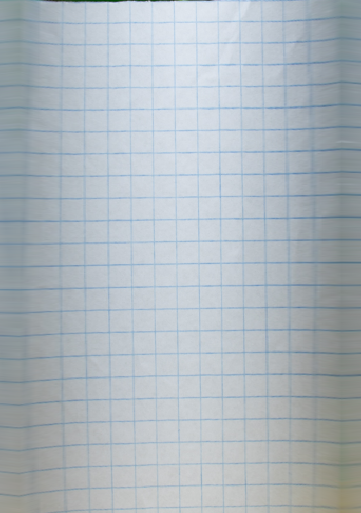
\includegraphics[width=.55\linewidth]{TCC/Imagens/ensaios/b_2020.png}
            \\
            (a) Imagem original & (b) Imagem planificada.
            \end{tabular}
        \fonte{O autor (2020).}
	\end{minipage}
    \label{fig:ensaio_2_2020a}
\end{figure}

\begin{figure}[ht]
    \caption{Resultado da planificação com N = 30.}     
    \centering
    \vspace{0.3cm}
    \begin{minipage}{.5\textwidth}
      \centering
            \begin{tabular}{cc}
            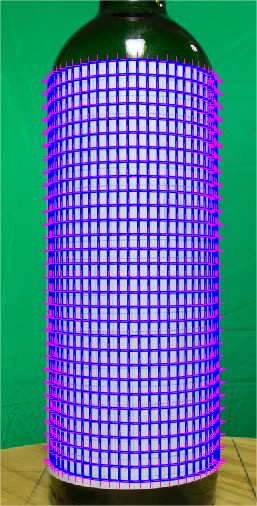
\includegraphics[width=.4\linewidth]{TCC/Imagens/ensaios/a_3030.jpg} 
            &
            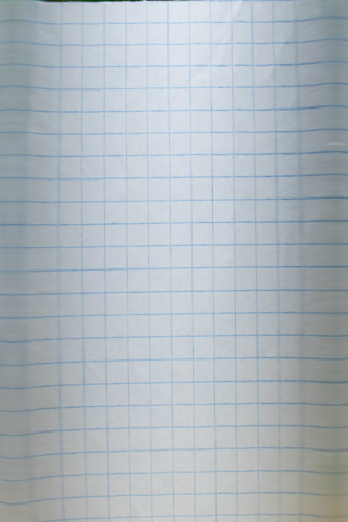
\includegraphics[width=.55\linewidth]{TCC/Imagens/ensaios/b_3030.png}
            \\
            (a) Imagem original & (b) Imagem planificada.
            \end{tabular}
        \fonte{O autor (2020).}
	\end{minipage}
    \label{fig:ensaio_2_3030a}
\end{figure}


Como mencionado, a utilização de uma maior quantidade de pontos de referência sobre a imagem resulta em um acréscimo significativo no custo computacional. 
Para realizar a medição de tempo necessário para cada execução, foi utilizada a ferramenta \textit{Profile} do MATLAB\textsuperscript{\tiny\textregistered}, que retorna a demanda de tempo em segundos de acordo com a utilização de cada método executado no código. Os valores de tempo analisados se atribuem somente ao método de planificação da imagem, desconsiderando o tempo de redimensionamento da imagem, tempo de alocação, etc. No gráfico disposto na Figura~\ref{fig:grafico_time} é demonstrado o tempo de execução do método de compensação das imagens de acordo com a quantidade de pontos.

\begin{figure}[ht]
    \caption{Tempo de execução (em segundos) para a quantidade de pontos total atribuída.}
    \centering
    \vspace{.3cm}
    \begin{minipage}{.7\textwidth}
        \hspace{.3cm}
        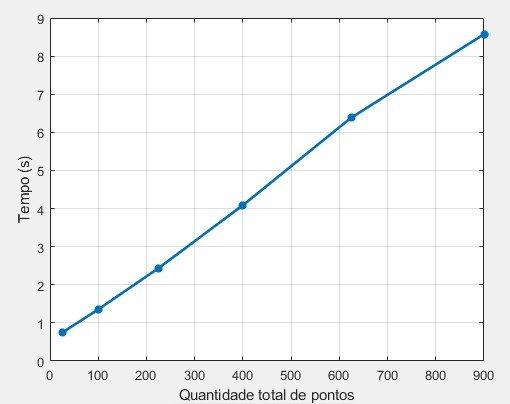
\includegraphics[width=\textwidth]{TCC/Imagens/ensaios/grafico.jpg}
        \fonte{O autor (2020).}
	\end{minipage}
    \label{fig:grafico_time}
\end{figure}

Observando-se o gráfico é possível afirmar que o tempo de execução cresce linearmente de acordo com o número de pontos atribuídos. A obtenção desses valores foi realizada seguindo as regras: execução de cinco realizações do algoritmo para cada valor de $N$, sendo considerada a média  dos valores de cada realização como o valor utilizado no gráfico; em cada uma das execuções, o comando \textit{clear all} era utilizado, a fim de evitar toda a pré-alocação de memória e outros fatores utilizados pela ferramenta para melhorar seu desempenho.

\section{Montagem da Panorâmica}

Nesta seção é avaliada a montagem da panorâmica considerando o movimento conhecido da garrafa. Como mencionado, esse sistema considera que a cena é espacialmente estática, ou seja, a garrafa e a câmera sempre vão estar fixas, realizando apenas o movimento de rotação 
da garrafa. A Figura~\ref{fig:panoramica} demonstra o resultado da montagem da panorâmica formada a partir das figuras dispostas em Figura~\ref{fig:figs_panoramica} (ver anexo A).

\begin{figure}[ht]
    \caption{Resultado da panorâmica cortando 45$^\circ$.}
    \centering
    \vspace{.3cm}
    \begin{minipage}{\textwidth}
    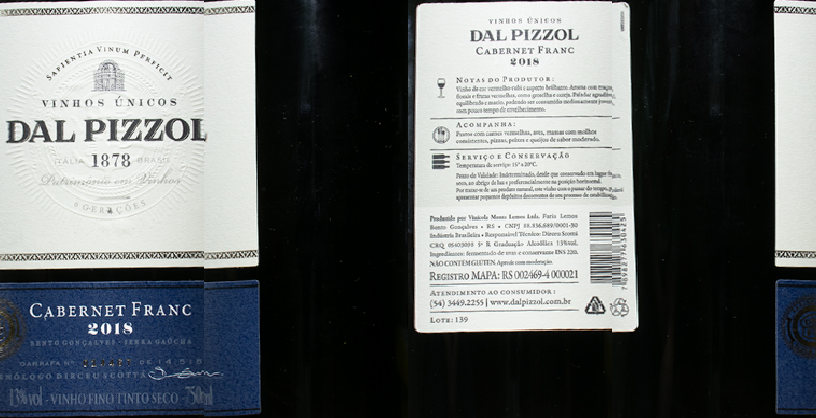
\includegraphics[width=\textwidth]{TCC/Imagens/result_45.png}
        \fonte{O autor (2020).}
	\end{minipage}
    \label{fig:panoramica}
\end{figure}

Cabe ressaltar a importância da precisão do sistema mecânico que compõe a solução proposta sistema. Visto que o local de costura do mosaico é facilmente identificável pelos diferentes níveis de iluminação nas imagens, para comentar os detalhes, cada quarto de imagem será nomeado como A, B, C e D, respectivamente. Nota-se pelas  regiões 
B e C que existe uma leve inclinação vertical no ponto de apoio da garrafa, o que interfere diretamente no alinhamento do sistema, que considera o posicionamento da garrafa como confiavelmente fixo, ou seja, quanto maior for o nível de controle do sistema mecânico, melhores podem ser os resultados obtidos através do método.

Neste resultado também é possível analisar que a desconsideração de 45º (1/4) em ambos os lados de cada imagem, apesar de terem sido utilizados valores teórico e ideais para o dimensionado aqui apresentado, resultou em uma boa representação de ponto de costura entre as imagens. Isto pode visto na junção do ''L'' (''em Pizzol''), bem como a extensão legível na parte inferior da costura entre os segmentos de imagem A e B.

Considerando que o presente trabalho conta com diversas ''não-idealidades'' para a implementação, o método conseguiu demonstrar através de uma única imagem todo o perímetro da garrafa, mesmo que com algumas falhas. Supondo um sistema mecânico superior em níveis de precisão, bem como o conhecimento dos principais
parâmetros da câmera que está sendo utilizada, os resultados de montagem da panorâmica podem ser melhorados a fim de corrigir pequenas imperfeições.


